% 
%  chapter1.tex
%  ThesisISEL
%  
%  Created by Serge Lage on 2019/07/30.
%
% ================
% = Blue Box =
% ================
\chapter{Blue Box}
\label{cha:blue_box}
This chapter explains the approach used to reach the first goal of this work. It describes an application that implements the work done in this chapter with respect to its functionality, architecture, implementation details and usage.  

\section{Introduction} % (fold)
\label{sec:introduction}
The first objective is to develop a locally implemented tool that informs whether the vessel is engaged in fishing, and if so, whether the fishing area is new or is habitually.\\
One of the solutions developed to meet this objective consists in a machine learning application to analyze data in real time, in order to determine whether the vessel is fishing, and if so, whether it is fishing in its fishing zone or in new location.\\
This solution must be implemented by vessel, therefore each vessel will only have access to its own data that is, each vessel only will know it’s one data.
The fact that this analysis is done by vessel allows avoiding bias in results, in fact each vessel has different power, size and its suitable for certain fishing activity.\\
This solution could be implemented and used as a library by the MONICAP system shown in \ref{fig:monicap} .\cite{WEBSITE:MonicapXsealence}.

\begin{figure}[H]
    \centering
    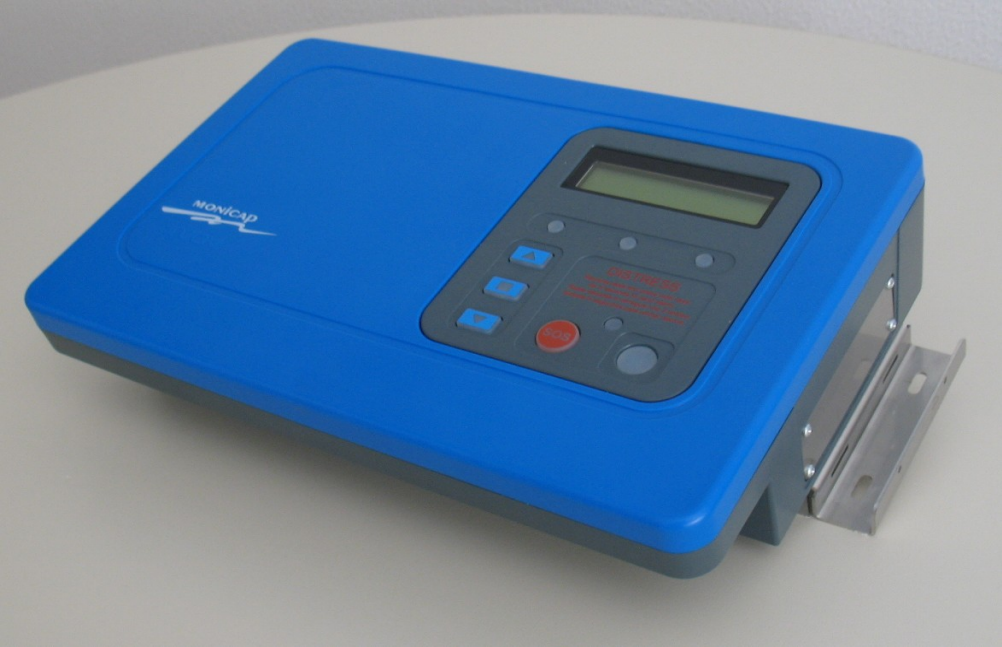
\includegraphics[width=0.8\linewidth]{Chapters/img/equipamento_monicap.png}
    \caption{MONICAP Blue Box.}
    \label{fig:monicap}
\end{figure}

As MONICAP systems are installed on ships, they can, in real time, send alerts to the authorities, whenever an abnormal change is detected in relation to the standard.

% section introduction (end)

\section{Fishing Velocity Patterns} % (fold)
\label{sub:fishing_velocity_patterns}
In order to know whether a vessel is fishing, we can use it’s velocity patterns, given that the speed of the vessel differs where it is travelling or when it is fishing. We can verify this fact in the plot shown in \ref{fig:histogram_vessel2} , corresponding to vessel with identification number 2.

On \ref{fig:histogram_vessel2} the histogram allows us to recognize two different velocity patterns, identified by two distinct distributions that are visible when we graphically represent the velocity’s data of each of the vessels. The distribution characterized by lower average speeds corresponds to fishing activity and the other speed distribution corresponds to the movement of the vessel between the port and the fishing sites.\\
So, it is needed to isolate the first distribution’s range to be able to classify the upcoming future velocity’s as fishing associated or not.
 
\begin{figure}[H]
    \centering
    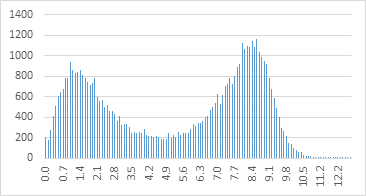
\includegraphics[width=0.8\linewidth]{Chapters/img/hist_vessel2.png}
    \caption{SOG Histogram vessel 2.}
    \label{fig:histogram_vessel2}
\end{figure}

In \ref{fig:histogram_vessel2} we have the speed in x axes in nautical knots and in the y axes the quantity of records per speed value.


To isolate the first distribution, it was used the Hill Climbing algorithm \cite{Kvasnicka1995HillCW}.  This algorithm is a local optimization algorithm which provides a direct search. The Stochastic Hill Climbing algorithm works supported in an iterate process of randomly selecting a neighbor for a candidate solution. The acceptance of the solution is conditioned by a criterion of improvement with respect to the previous solution.\\
The implementation used was altered in a way that when the algorithm converges to the maximum, it will continue to find the limit of the distribution.
To obtain this solution, the algorithm searches for the first local maximum that does not have a higher value in the following three points (current key + 0.5, current key + 1 and current key + 2), in this way we can find the maximum value of the fishing speed range. \\
To find the end of the fishing speed range, the algorithm continues to sweep the histogram until the next three points are not lower than the current point.
This way we can end up with a histogram of the intended distribution as we can observe in  \ref{fig:sog_hill_climbing}.

\begin{figure}[H]
    \centering
    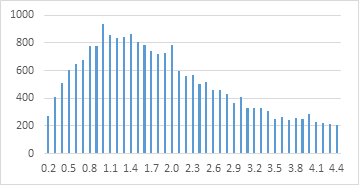
\includegraphics[width=0.8\linewidth]{Chapters/img/sog_hill_climbing.png}
    \caption{Velocity distribution of vessel 2 after the application to the Hill Climbing algorithm}
    \label{fig:sog_hill_climbing}
\end{figure}

Once the distribution corresponding to the fishing speeds has been identified the next step is to define a range to classify the new data, a minimum speed and a maximum speed.
Inside this range we classify the vessel as fishing. With this purpose were considered three optional procedures:
\begin{itemize}
\item	\textbf{Standard devariation:}
This solution assume that the velocity distribution is a normal distribution.   Using the distribution of the fishing velocity we find the fishing velocity with more occurrences and with the standard devariation we can chose a distance from mean and so we can get the minimum population desired (explained by Chebyshev’s inequality \cite{Chebyshevinequality}) to be within the fishing range. 

\item	\textbf{Kernel Density Estimation:}
Kernel Density Estimation method estimates the probability density function by imposing a model function on every data point and then adding them together. The function applied to each data point is called a kernel function \cite{KernelDensityEstimation}.

\item	\textbf{Filter:}
Using a filter that remove all the velocity occurrences that happens less than 10 \% of the maximum occurrence and isolating the occurrences that are fallowed we can retrieve a clean distribution of the fishery speed of that vessel.  With this we can use the first and last values to classify the new inputs. To isolate the fishery speed, I use a hill climb algorithm, assuming that the first distribution is the fishery speed.
\end{itemize}

The used procedure was performed in two parts:  it starts by using the method based in the \textbf{Filter} to isolate the fishery speed from the remain. Then the Kernel distribution method was applied.
\begin{enumerate}


\item	\textbf{Filter:} In the first step it retrieves all velocity data from the database to create a histogram like is shown in the \ref{fig:histogram_vessel2} . In the next step it uses the hill climbing algorithm to get the minimum and the maximum value of the first distribution. The velocity 0 is removed because we don’t want to consider when the vessel is completely stopped. 
\item	\textbf{Kernel:} It was applied a kernel distribution method in the filtered histogram to have the distribution represented in orange on \ref{fig:hist_kernel}. The it was created a dictionary with the velocity’s and the cumulative percentage of velocity. This way we end up with a histogram like \ref{fig:hist_comulative}.  
Then a range across quantiles is defined for some probability. As in the estimation of confidence intervals, a confidence level is also defined here, to which will be associated the two speed limits that correspond to the fishing activity.
\end{enumerate}  

\begin{figure}[H]
    \centering
    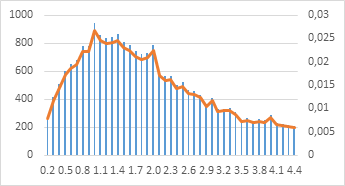
\includegraphics[width=0.8\linewidth]{Chapters/img/hist_kernel.png}
    \caption{Kernel distribution filtered data}
    \label{fig:hist_kernel}
\end{figure}


Now we can compare the new data with the established limits. If the new data is within the limits, we classify as fishing, if not, we classify as not fishing.

\begin{figure}[H]
    \centering
    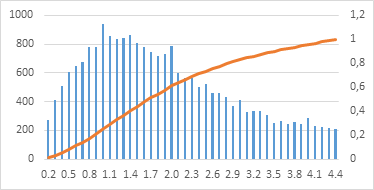
\includegraphics[width=0.8\linewidth]{Chapters/img/hist_comulative.png}
    \caption{Filtred histogram with comulative kernel distribution}
    \label{fig:hist_comulative}
\end{figure}


% section fishing_velocity_patterns (end)


\section{Fishing Spots} % (fold)
\label{sub:fishing_spots}

Using the history of GPS locations by vessel, in this point to decide whether the vessel is fishing in its fishing zone or in a new location.
Fishing in a new zone may mean that the vessel has change its type of fishing or is engaging in an activity that is not licensed.


\begin{figure}[H]
    \centering
    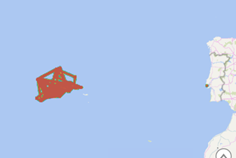
\includegraphics[width=0.8\linewidth]{Chapters/img/gps_vessel2.png}
    \caption{Vessel 2 GPS points}
    \label{fig:gps_vessel2}
\end{figure}

In \ref{fig:gps_vessel2} we can see the GPS points of a vessel. Using methods based in clustering it is possible to identify several areas by vessel that are the normal fishing zones of the vessel. When the vessel is outside that zone, a flag should occur.

Using the fishing velocity range encountered in the previous point, we get the GPS points of the vessel within that range, so we can work only with the positions where the vessel was fishing. The next step is to use a clustering algorithm to define the fishing areas, so we can compare with the new GPS points. 

For this purpose, diverse data mining algorithms were performed in order to choose the best results:

\begin{itemize}
\item	\textbf{K-Means:}
K-means clustering algorithm \cite{HitchcockKmeans} is a method of cluster analysis which aims the partition of n observations into k clusters in which each observation belongs to the cluster with the nearest mean. This results into a partitioning of the data space. K-means (Macqueen, 1967) is one of the simplest unsupervised learning algorithms that solve the well-known clustering problem. The procedure follows a simple and easy way to classify a given data set through a certain number of clusters (assume k clusters) fixed a priori. The main idea is to define k centroids, one for each cluster. These centroids should be placed in a cunning way because of different location causes different result. So, the better choice is to place them as much as possible far away from each other. The next step is to take each point belonging to a given data set and associate it to the nearest centroid. When no point is pending, the first step is completed, and an early group is done. At this point we need to recalculate k new centroids as bar centers of the clusters resulting from the previous step. After we have these k new centroids, a new binding must be done between the same data set points and the nearest new centroid. A loop has been generated. As a result of this loop we may notice that the k centroids change their location step by step until no more changes are done.

 
\item	\textbf{Density Based Cluster:}
Density-based clustering algorithms \cite{WekaCC} try to find clusters based on the estimation of the density of data points in a region.
It can find arbitrarily shaped clusters and handles noises and yet is a one-scan algorithm that needs to examine the raw data only once. In density-based clustering algorithms, dense areas of objects in the data space are considered as clusters, which are segregated by low-density area (noise). The basic idea of density-based clustering is clusters are dense regions in the data space, separated by regions of lower object density \cite{WEKATalankiDensity}.
The key idea of density-based clustering is that for each instance of a cluster the neighborhood of a given radius (Eps) must contain at least a minimum number of instances (Min Pts).

\item	\textbf{DBSCAN:}
DBSCAN (for density-based spatial clustering of applications with noise) is a data clustering algorithm proposed by Martin Ester, Hans-Peter Kriegel, Jorge Sander and Xiaowei Xu in 1996 It is a density-based clustering algorithm because it finds a number of clusters starting from the estimated density distribution of corresponding nodes. DBSCAN \cite{Kisilevich2010PDBSCANAD} is one of the most common clustering algorithms and most cited in scientific literature.
\end{itemize}

After some tests it was decided that Density Based Cluster is the best approach for this case. It was excluded DBSCAN, because as we can observe in \ref{table:mill_per_moodle}, this model needs a lot of processing power to estimate the clusters. These values were retrieved using a computer with an Intel i5 (2.5 GHz) and 8 GB of RAM. Considering that the Blue Box as a lot less processing power it was decided that this model is not a good solution for this problem.
\\

\begin {table}[H]
\begin{center}
\begin{tabular}{c|c|c|c}
             & \textbf{K-Means} & \textbf{Density Based Cluster} & \textbf{DBSCAN} \\
\hline
Initializing & 862              & 923                             & 25848           \\

New data     & 25               & 45                            & 35  
           
\label{table:mill_per_moodle}
\end{tabular}
\caption {Milliseconds per model}
\end{center}
\end {table}

The choice between K-Means and Density Based Cluster algorithms was based in the fact that Density Based Cluster represents a great advantage because it estimates the probability of the new GPS point belonging to a cluster based in the cluster probabilistic distribution. So that way the user can set what is the best configuration. The clusters themselves are equal between K-Means and Density Based Cluster since Density Based Cluster uses K-Means to define the centroids, only differ by adding a layer to define the area of density per cluster.
\\
In order to decide the number of clusters it was used the elbow method \cite{Kodinariya2013ReviewOD}, for the within cluster sum of squares, as could be seen in \ref{fig:elbow_method}. The within means the distance the vectors in each cluster are from their respected centroid. The goal is to get this number as small as possible. One approach to handling such objective is to run the kmeans clustering multiple times, raising the number of the clusters each time. Then it is possible to compare the withinss each time, stopping when the rate of improvement drops off. The better case corresponds to find a low withinss while still keeping the number of clusters low.\\
The elbow method is a visual method. The idea is that Start with K=2, and keep increasing it in each step by one unit, calculating the clusters and the cost that comes with the training. At some value for K the cost drops dramatically, and after that it reaches a plateau when you increase it further. This is the K value we want. We can observe that six clusters are a good number as the error is not decreasing much as the number of clusters increases. To exemplify the data used in \ref{fig:elbow_method} was the GPS points of all vessels.


\begin{figure}[H]
    \centering
    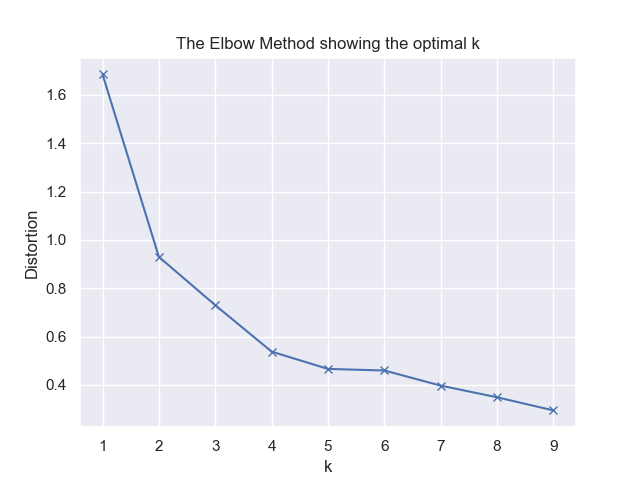
\includegraphics[width=0.8\linewidth]{Chapters/img/elbow_method.png}
    \caption{Sum of squared error by number of clusters}
    \label{fig:elbow_method}
\end{figure}



% section fishing_spots (end)



\section{DSA Library} % (fold)
\label{sub:dsa_library}


It was created a software application called DSALib for (Decision Support Alerts Library). In this application it was applied the solutions described in this chapter to help with the elaboration and tests for this project. For a market solution this library could be used by the main application of MONICAP to send alerts to support decision making or to simply classify each VMS data entry as if fishing and if fishing in a new area for future analysis .

\newpage


\subsection{Functionality} % (fold)
\label{sub:functionality}

This application makes it possible to:
\begin{itemize}
\item Test new data \\ Send vms data and recive if is considred to be fishing and if is in new area.
\item Test new velocity \\ Send sog data and recive true if is considred to be fishing.
\item Test new location \\ Send GPS data and recive true if is in new area.
\item Restart models \\ Request to create new models. Can be used if the object is running for a long time and want to renew models with new data. 
\item Get limits \\ Request the velocity limits. Receve a tuple with two doubles (item1 = low speed limit, item2 = high speed limit). Can be used for analisys like in chapter 5.
\end{itemize}

To make this possible is necessary to configure the data access layer to get the vms data from the local data repository.
Correnlty, the application supports conection to SQL Server \cite{WEBSITE:SqlServer} and PostgreSQL \cite{WEBSITE:Postgresql}.


% subsection functionality (end)


\subsection{Architecture and Implementation} % (fold)
\label{sub:architecturee_implementation}
To develop the software, I decided to use Java 8 \cite{WEBSITE:OraJava8} because it is a powerful, full object-oriented and cross-platform programming language. MONICAP uses Linux so using a JRE (Java Runtime Environment) application is a good choice.
The architeture is depiced in \ref{fig:DSALib_Prof}. In this architeture is possible to distiguish three main modules: One that is the core of the DSALib, create the modules and use them. Other one is WEKA \cite{WEBSITE:Weka} that create de cluster modules for locations and kernel density for velocity. The last one is the data access layer that is responsible to get the vms data from the local repository so DSALib can create the modules.


\begin{figure}[h]
    \centering
    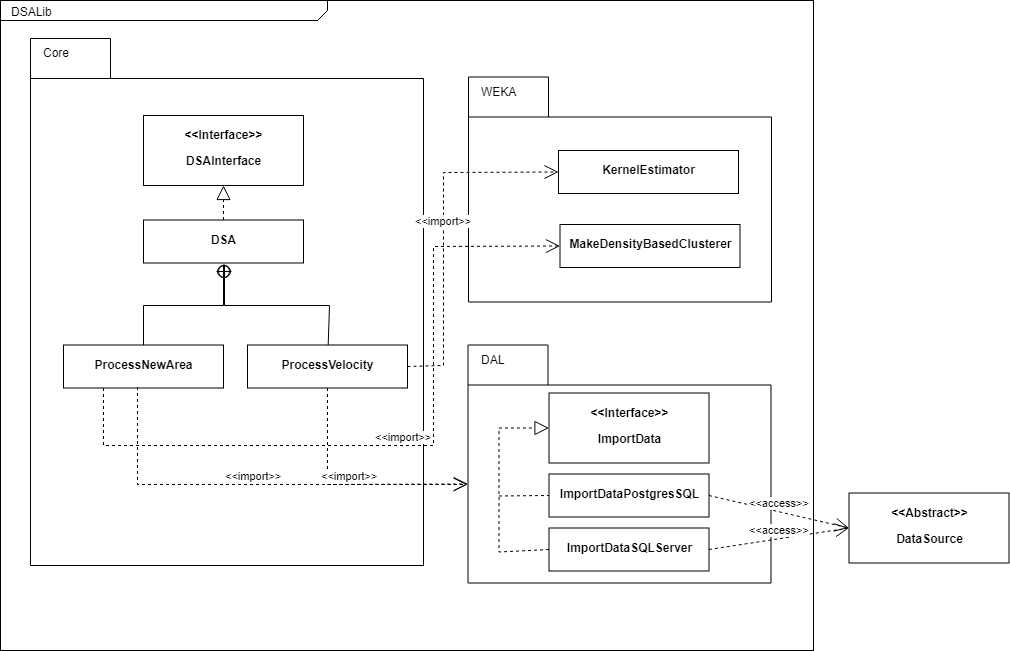
\includegraphics[width=1.0\linewidth]{Chapters/img/DSALib_Prof.png}
    \caption{Representation of the DSALib architecture.}
    \label{fig:DSALib_Prof}
\end{figure}



\textbf{Core module} \\The core module is responsible to initialize the models and use them the way discribed in this chapter. It starts by creting an instace of ProcessVelocity to create de first model and then create an instece of ProcessNewArea that uses the velocity limits previously obtained to get the locations data form when the vessel was fishing to create the module.

\textbf{WEKA module} \\Weka is a collection of machine learning algorithms for data mining tasks. It contains tools for data preparation, classification, regression, clustering, association rules mining, and visualization. In this application, WEKA is used as a tool to create the modules.

\textbf{DAL module} \\The data access module was implemented in an way not only to get data but also to filter data in the database engine. Filtering data (where) is optimized on the database engine and so we gain some performance.




The application starts by initializing two objects:
\begin{enumerate}
\item	ProcessVelocity: This object is responsible to do the process explained in the point 4.2 of this document. This object will request to the static class ImportData to retrieve all SOG (Speed Over Ground) data from the database. Then the process will end with the limits (minimal speed of fishing and the maximal speed of fishing).
\item	ProcessNewArea: This object is responsible to do the process explained in the point 4.3 of this document. This object is only initialized after ProcessVelocity because it needs the velocity fishing limits to only create the clusters of the fishing areas. With these limits the object request to ImportData only the Lat and Lon where the vessel was in between the velocity limits. With this the object ends up with the clusters of the fishing areas.
\end{enumerate}


Output newData(Input input);
boolean isFishing(double velocity);
boolean isNewArea(GPS gps);
void restart();
Limits GetLimit(); 
% subsection architecturee_implementation (end)

\subsection{Usage} % (fold)
\label{sub:usage}
To use we start by instantiate DSALib with the doubles limitVelociry and limitArea. This doubles range between 0 and 1:
\begin{itemize}
\item	limitVelociry: used to get the maximum and minimum speed by reducing the speed range. This limit will reduce de maximum speed and increase the minimum speed by setting the maximum velocity as the velocity that as (1-limit) percentage of the cumulative karnel distribution and the minimum velocity as the velocity that as (limit) percentage of the cumulative karnel distribution.
\item	limitArea: used to compare with the probability to belong in a cluster given to the new points. If the limit is smaller that the given probability, then the vessel is classified as fishing in a new area.
\end{itemize}
These limits are important so we can configure if we prefer to have more false positive or false negative classifications.
A false positive (type I error) is when the classifier reject a true hypothesis.
A false negative (type II error) is when the classifier accept a false hypothesis.

After we have the DSALib ready we need to send a new velocity data and GPS coordinates to receive an object with an “isFishing” as true if the vessel is fishing and an “isNewArea” as true if the vessel is in an area that is not a normal fishing area and it’s in a fishing velocity. In Appendix B there is more information about the software developed.

% subsection usage (end)

% section dsa_library (end)
% chapter blue_box (end)



